\chapter{Implementacija i korisničko sučelje}
		
		
		\section{Korištene tehnologije i alati}
		
			\textbf{\textit{dio 2. revizije}}
			
			 \textit{Detaljno navesti sve tehnologije i alate koji su primijenjeni pri izradi dokumentacije i aplikacije. Ukratko ih opisati, te navesti njihovo značenje i mjesto primjene. Za svaki navedeni alat i tehnologiju je potrebno \textbf{navesti internet poveznicu} gdje se mogu preuzeti ili više saznati o njima}.
			 
			 Za potrebe rada na projektu, tim je komunicirao preko aplikacija WhatsApp\footnote{https://www.whatsapp.com/} i Discord\footnote{https://discord.com/}. 
			 Za izradu UML dijagrama, korišten je alat Astah\footnote{https://astah.net/}.
			 Za upravljanje različitim verzijama datoteka korišten je sustav Git\footnote{https://git-scm.com/}.
			 Udaljeni repozitorij projekta nalazi se na platformi Github\footnote{https://github.com/}. Za izradu i testiranje baze korišten je sustav za upravljanje bazama podataka PostgreSQL\footnote{https://www.postgresql.org/}.
			 
			 Kao integrirano razvojno okruženje (IDE) korišten je Intellij IDEA\footnote{https://www.jetbrains.com/idea/}. Ovaj IDE razvio je JetBrains. Koristi se prvenstveno za razvoj softvera napisanog u Javi, Kotlinu i drugim JVM (Java Virtual Machine) jezicima. Preko pluginova nudi podršku i za mnoge druge programske jezike kao što su Python, R, Julia itd. Za potrebe rada na projektu, tim je koristio studentske licence za navedeni IDE preko kojih je moguće koristiti podršku Intellij-a za razne radne okvire (npr. Spring, React).
			 
			 Aplikacija \textit{Ozdravi} napisana je koristeći radni okvir React\footnote{https://react.dev/} za \textit{frontend} te radni okvir Spring\footnote{https://spring.io} za \textit{backend}.
			 \textit{React} je Javascript biblioteka otvorenog koda za izradu korisničkih sučelja. Održavaju ju Meta i zajednica programera i tvrtki. Ova biblioteka brza je i jednostavna za koristiti te se pomoću nje najčešće razvijaju single-page aplikacije. Velika prednost toga je što React omogućuje da se prilikom korištenja sučelja ponovno naslikaju (renderaju) samo dijelovi koji su se izmijenili. Sučelje izrađeno pomoću Reacta sastavljeno je od komponenti koje se mogu ponovno iskoristiti.
			 \textit{Spring} je besplatan radni okvir za razvoj aplikacija u Javi (i drugim jezicima). Vrlo je popularan zbog različitih modula koje nudi čime se znatno ubrzava stvaranje aplikacije. U sklopu izrade ove aplikacije korišteni su Spring Boot (razvoj aplikacije s minimalnom količinom konfiguracija), Spring Security (jednostavna konfiguracija zaštite aplikacije), Spring Data JPA (za lakšu komunikaciju s bazom podataka) i drugi. Za brzo početno podešavanje korištena je stranica Spring initializr\footnote{https://start.spring.io/}.
				
			
			\eject 
		
	
		\section{Ispitivanje programskog rješenja}
			
			\textbf{\textit{dio 2. revizije}}\\
			
			 \textit{U ovom poglavlju je potrebno opisati provedbu ispitivanja implementiranih funkcionalnosti na razini komponenti i na razini cijelog sustava s prikazom odabranih ispitnih slučajeva. Studenti trebaju ispitati temeljnu funkcionalnost i rubne uvjete.}
	
			
			\subsection{Ispitivanje komponenti}
			\textit{Potrebno je provesti ispitivanje jedinica (engl. unit testing) nad razredima koji implementiraju temeljne funkcionalnosti. Razraditi \textbf{minimalno 6 ispitnih slučajeva} u kojima će se ispitati redovni slučajevi, rubni uvjeti te izazivanje pogreške (engl. exception throwing). Poželjno je stvoriti i ispitni slučaj koji koristi funkcionalnosti koje nisu implementirane. Potrebno je priložiti izvorni kôd svih ispitnih slučajeva te prikaz rezultata izvođenja ispita u razvojnom okruženju (prolaz/pad ispita). }
			
			
			
			\subsection{Ispitivanje sustava}
			
			 \textit{Potrebno je provesti i opisati ispitivanje sustava koristeći radni okvir Selenium\footnote{\url{https://www.seleniumhq.org/}}. Razraditi \textbf{minimalno 4 ispitna slučaja} u kojima će se ispitati redovni slučajevi, rubni uvjeti te poziv funkcionalnosti koja nije implementirana/izaziva pogrešku kako bi se vidjelo na koji način sustav reagira kada nešto nije u potpunosti ostvareno. Ispitni slučaj se treba sastojati od ulaza (npr. korisničko ime i lozinka), očekivanog izlaza ili rezultata, koraka ispitivanja i dobivenog izlaza ili rezultata.\\ }
			 
			 \textit{Izradu ispitnih slučajeva pomoću radnog okvira Selenium moguće je provesti pomoću jednog od sljedeća dva alata:}
			 \begin{itemize}
			 	\item \textit{dodatak za preglednik \textbf{Selenium IDE} - snimanje korisnikovih akcija radi automatskog ponavljanja ispita	}
			 	\item \textit{\textbf{Selenium WebDriver} - podrška za pisanje ispita u jezicima Java, C\#, PHP koristeći posebno programsko sučelje.}
			 \end{itemize}
		 	\textit{Detalji o korištenju alata Selenium bit će prikazani na posebnom predavanju tijekom semestra.}
			
			\eject 
		
		
		\section{Dijagram razmještaja}
			
			\textbf{\textit{dio 2. revizije}}
			
			 \textit{Potrebno je umetnuti \textbf{specifikacijski} dijagram razmještaja i opisati ga. Moguće je umjesto specifikacijskog dijagrama razmještaja umetnuti dijagram razmještaja instanci, pod uvjetom da taj dijagram bolje opisuje neki važniji dio sustava.}
			 
			 Dijagram razmještaja je strukturni UML dijagram koji opisuje topologiju sustava i prikazuje odnos sklopovskih i programskih dijelova. Na slici \ref{fig:dijagramrazmjestaja} prikazan je specifikacijski dijagram razmještaja aplikacije. Na čvoru koji predstavlja korisnički uređaj nalazi se web preglednik (artefakt) korisnika. On preko HTTPS protoka komunicira s poslužiteljem. Poslužitelj pruža uslugu poslužitelja frontenda, backenda te baze podataka. Sve te usluge mogu međusobno komunicirati slanjem zahtjeva.
			 
			 \begin{figure}[H]
			 	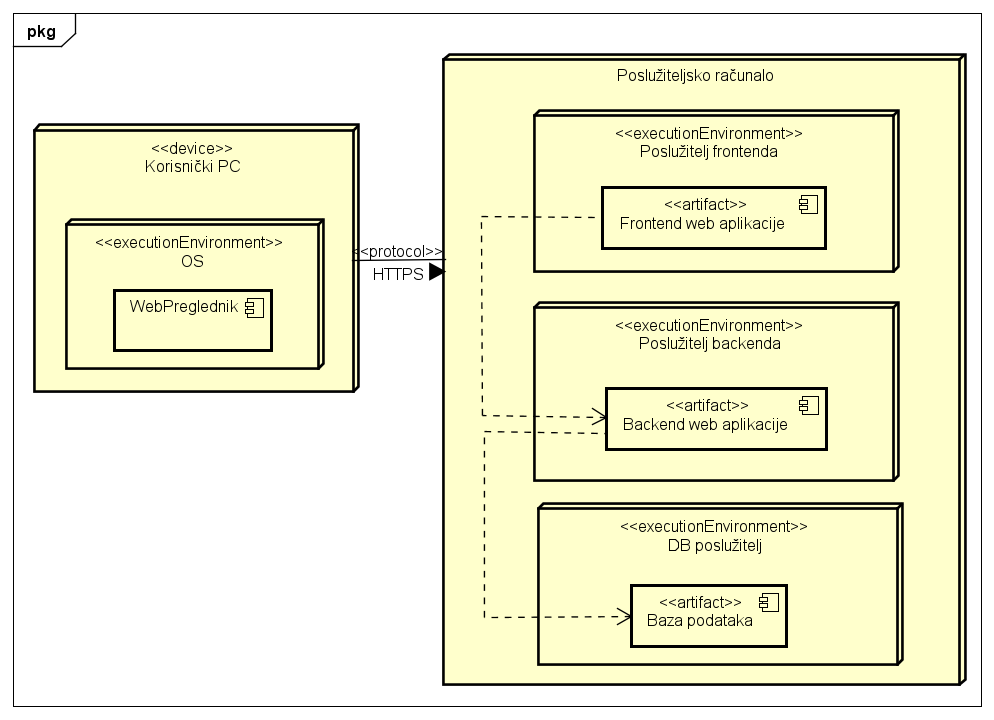
\includegraphics[width=\textwidth]{dijagrami/Dijagram razmjestaja.PNG} %veličina u odnosu na širinu linije
			 	\caption{Dijagram razmještaja}
			 	\label{fig:dijagramrazmjestaja} %label mora biti drugaciji za svaku sliku
			 \end{figure}
			
			\eject 
		
		\section{Upute za puštanje u pogon}
		
			\textbf{\textit{dio 2. revizije}}\\
		
			 \textit{U ovom poglavlju potrebno je dati upute za puštanje u pogon (engl. deployment) ostvarene aplikacije. Na primjer, za web aplikacije, opisati postupak kojim se od izvornog kôda dolazi do potpuno postavljene baze podataka i poslužitelja koji odgovara na upite korisnika. Za mobilnu aplikaciju, postupak kojim se aplikacija izgradi, te postavi na neku od trgovina. Za stolnu (engl. desktop) aplikaciju, postupak kojim se aplikacija instalira na računalo. Ukoliko mobilne i stolne aplikacije komuniciraju s poslužiteljem i/ili bazom podataka, opisati i postupak njihovog postavljanja. Pri izradi uputa preporučuje se \textbf{naglasiti korake instalacije uporabom natuknica} te koristiti što je više moguće \textbf{slike ekrana} (engl. screenshots) kako bi upute bile jasne i jednostavne za slijediti.}
			
			
			 \textit{Dovršenu aplikaciju potrebno je pokrenuti na javno dostupnom poslužitelju. Studentima se preporuča korištenje neke od sljedećih besplatnih usluga: \href{https://aws.amazon.com/}{Amazon AWS}, \href{https://azure.microsoft.com/en-us/}{Microsoft Azure} ili \href{https://www.heroku.com/}{Heroku}. Mobilne aplikacije trebaju biti objavljene na F-Droid, Google Play ili Amazon App trgovini.}
			
			
			\eject 